\newpage
	\section{S} \label{sec:S}

		\subsection{SCALABILITÀ} \index{Scalabilità} \label{scalabitlita}
		È la caratteristica di un sistema software o hardware facilmente modificabile nel caso di variazioni notevoli della mole o della tipologia dei dati trattati. \\
		Garantisce prestazioni.


		\subsection{SEMAT} \index{SEMAT} \label{semat}
		\textit{Software Engineering Method and Theory} fornisce teorie, principi provati e \underline{\hyperref[best]{best practices}} per l'Ingegneria del Software.


		\subsection{SISTEMA DI QUALITÀ} \index{Sistema di qualità} \label{sistemadiqualita}
		Riferimenti \textbf{oggettivi} che ci dicono come stiamo lavorando.


		\subsection{SLACK} \index{Slack} \label{slack}
		Significato letterale:``lasco''. Con questo si intende il margine che posso consumare (per esempio, nel caso di un ritardo di attività che devo finire di completare).


		\subsection{SOFTWARE DETERMINISTICO} \index{Software deterministico} \label{softwaredeterministico}
		In ogni stato del prodotto SW in cui mi trovo, so che posso avere solo ``un'unica e sola uscita''. Devo sempre sapere lo stato in cui sono, quindi avere ben chiaro quello precedente e quello seguente.


		\subsection{SOFTWARE ENGINEERING} \index{Software Engineering} \label{swe}
		 L'\underline{\hyperref[engineering]{Ingegneria}} del Software è una disciplina volta a realizzare  \underline{\hyperref[prodotto]{prodotti software}} talmente impegnativi da richiedere lo svolgimento di attività collaborative. Agisce garantendo \underline{\hyperref[efficacia]{efficacia}} ed \underline{\hyperref[efficienza]{efficienza}} durante tutto il \underline{\hyperref[ciclo]{ciclo di vita}} del prodotto. \\
		 È importante sottolineare che l'Ingegneria del Software non ha a che vedere solo con l'informatica, ma anche con alcune aree della matematica discreta, ricerca, statistica, psicologia ed economia. L'Ingegneria del Software inoltre adotta un determinato \underline{\hyperref[approccio]{approccio}}.


		\subsection{SOFTWARE SYSTEM} \index{Sistema software} \label{sistemasoftware}
		Soluzione realizzabile (concretizza \underline{\hyperref[requirements]{requirements}}).


		\subsection{SOLUTION} \index{Solution} \label{solution}
		Secondo elemento di un \underline{\hyperref[progetto]{progetto}} secondo \underline{\hyperref[semat]{SEMAT}}. Esso comprende \underline{\hyperref[requirements]{requirements}} e
		 \underline{\hyperref[sistemasoftware]{software system}}.

		\subsection{STAKEHOLDER} \index{Stakeholder} \label{stakeholder}
		Traduzione di \textit{portatori di interesse}, sono le persone influenti per il prodotto: dicono se una certa \underline{\hyperref[opportunity]{opportunità}} è buona.
		Possono essere chi usa il prodotto (cliente), chi compra il prodotto (committente), chi sostiene i costi di realizzazione (fornitore), chi verifica l'attuazione di processi (eventuali regolatori). \\
		È uno degli elementi di un progetto (vedi \underline{\hyperref[customerimage]{immagine}}).

		\subsection{STANDARD DI PROCESSO} \index{Standard di processo} \label{standard}
		Nascono per iniziativa del committente al fine di facilitare controllo, collaudo e accettazione.
		Esistono standard come:
		\begin{itemize}
			\item \textbf{Modello di azione}: definiscono procedure o processi
			\item \textbf{Modello di valutazione}: sono modelli più generali e identificano la \underline{\hyperref[best]{best practice}}
		\end{itemize}


			\subsubsection{STANDARD IEEE 830-1998}	\index{Standard IEEE 830-1998} \label{ieee830}
			Questo standard delinea la struttura che deve avere il documento \underline{\hyperref[analisideirequisiti]{Analisi dei Requisiti}} e le \underline{\hyperref[qualita]{qualità}} che devono possedere i requisiti.
			\textit{Recommended Practice for Software Requirements Specifications} dice che la specifica deve essere:
				\begin{itemize}
					\item Priva di ambiguità
					\item Corretta
					\item Completa
					\item Verificabile
					\item Consistente
					\item Modificabile
					\item Tracciabile
					\item Ordinata per rilevanza
				\end{itemize}
			Per la restante documentazione relativa alla struttura dell'AdR, vedere il \href{https://www.cs.purdue.edu/homes/apm/courses/BITSC461-fall03_SoftwareEngineering/miller-guidelines/IEEE830-1998.html}{link qui}.


			\subsubsection{STANDARD ISO 12207}	\index{Standard ISO 12207}	\label{12207}
			È un \textit{modello di azione} ed il modello più noto. Contiene tutti i processi significativi ad alto livello:
			\begin{itemize}
				\item Identifica i processi di ciclo di vita del \underline{\hyperref[prodotto]{software}}
				\item Ha struttura modulare
				\item Specifica le responsabilità sui processi
				\item Specifica i prodotti dei processi
			\end{itemize}

			\begin{figure}[H]
				\centering
				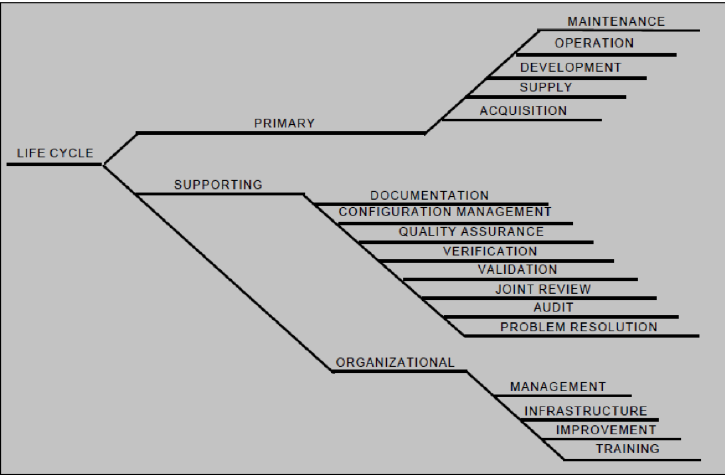
\includegraphics[width=0.78\textwidth]{img/iso}
				\caption{Primary, supporting and organisational life-cycle processes.}
			\end{figure}

			Almeno un \textit{processo primario} deve sempre esistere:
				\begin{itemize}
					\item \textbf{Acquisizione}: gestione dei sotto-fornitori
					\item \textbf{Fornitura}: gestione dei rapporti con il cliente
					\item \textbf{Sviluppo}: non è sempre detto che abbia rapporti con il cliente
					\item \textbf{Gestione operativa/utilizzo}: installazione ed erogazione dei prodotti
					\item \textbf{\underline{\hyperref[manutenzione]{Manutenzione}}}
				\end{itemize}

			\textit{Processi di supporto}:
				\begin{itemize}
					\item \textbf{Documentazione}
					\item \textbf{Accertamento della \underline{\hyperref[qualita]{qualità}}}
					\item \textbf{Gestione delle \underline{\hyperref[versione]{versioni}} e delle \underline{\hyperref[configurazione]{configurazioni}}}
					\item \textbf{\underline{\hyperref[verificare]{Verifica}}}
					\item \textbf{\underline{\hyperref[validare]{Validazione}}}
					\item \textbf{Revisioni congiunte con il cliente}
					\item \textbf{Verifiche ispettive interne}
					\item \textbf{Risoluzione dei problemi}: con gestione dei problemi
				\end{itemize}

			Trasversali rispetto ai singoli progetti sono invece i \textit{processi organizzativi}:
				\begin{itemize}
					\item \textbf{Gestione dei processi}
					\item \textbf{Gestione delle infrastrutture}
					\item \textbf{Miglioramento del processo}
					\item \textbf{Formazione del personale}
				\end{itemize}

			%La soluzione dei problemi... problem solution.	%slide 10/22


			\subsubsection{STANDARD ISO 14598}	\index{Standard ISO 14598}	\label{14596}
			ISO/IEC 14598:1999 fornisce il \textit{modello di valutazione} che non cambia nel tempo e col contesto. La metrica che adotta è un modo
			%per mettere in scala i numeri,
			per dare un significato condiviso e non ambiguo a delle caratteristiche.


			\subsubsection{STANDARD ISO 15504}	\index{Standard ISO 15504}	\label{15504}
			\textit{Software Process Improvement Capability dEtermination} \\
			Standard di \underline{\hyperref[qualita]{qualità}} nato per armonizzare 12207 e 9001. È un \textit{modello di valutazione} e si occupa di:
			\begin{itemize}
				\item \textbf{Identificazione degli stakeholder}: destinatari dei risultati, responsabili dei processi valutati
				\item \textbf{Scelta tra valutazione e miglioramento}: risultato a uso esterno o interno, approccio formale (\underline{\hyperref[audit]{\textit{audit}}}) o meno (\textit{self-assessment})
				\item \textbf{Definizione della portata}: processi inclusi nella valutazione e indicatori di valutazione
			\end{itemize}


			\subsubsection{STANDARD ISO 15939}	\index{Standard ISO 15939}	%slide 10 - Misurazione del software
			(Sappiamo solo che esiste ma non è da usare perchè è costoso) \\
			Misura e ha forma di ciclo, quindi non ha fine.
			%Si passa sempre per il punto di Management processes.
			Il mio cruscotto cambia in base al contesto, non è scelto a priori e basta, se no diventa vecchio (esempio: quando faccio codice guardo la qualità per il codice, quando faccio requisiti ho un altro cruscotto).


			\subsubsection{STANDARD ISO 25000}	\index{Standard ISO 25000}	\label{2500}
			ISO/IEC 25000:2014 è un insieme dello standard 9126 e 14598.
			Si riferisce al software, \textit{SQuaRE}: \textit{Software product Quality Requirements and Evaluation}.


			\subsubsection{STANDARD ISO 9000}	\index{Standard ISO 9000}	\label{9000}
			La famiglia delle norme ISO 9000 tratta i fondamenti dei modelli di qualità, neutri rispetto al dominio di applicazione.

			\begin{figure}[H]
				\centering
				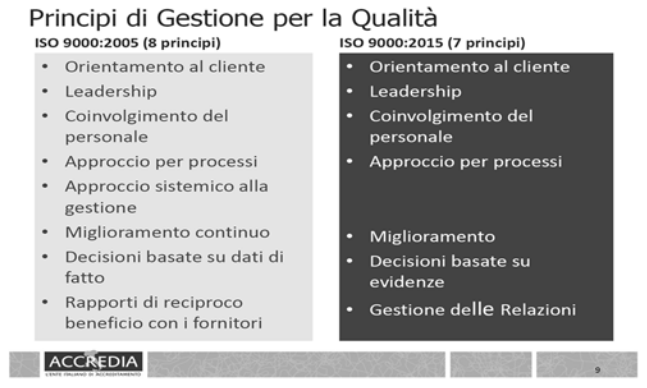
\includegraphics[width=0.65\textwidth]{img/9000}
				\caption{I principi ISO 9000.}
			\end{figure}


			\subsubsection{STANDARD ISO 9001}	\index{Standard ISO 9001}	\label{9001}
			Applica lo standard 9000 ai sistemi produttivi. È la certificazione per la valutazione dei fornitori di prodotti o servizi. \\
			Per il miglioramento dei risultati è stato in seguito creato il 9004.


			\subsubsection{STANDARD ISO 9126}	\index{Standard ISO 9126}	\label{9126} % slide 13/22 Set Qualità
			Standard per la qualità del prodotto.
			Fatto di due parti:
				\begin{itemize}
					\item Come si definiscono le caratteristiche rilevanti
					\item Come si misurano (con quali \underline{\hyperref[metrica]{metriche}}) per poterle valutare
				\end{itemize}
			Tre diverse visioni tutte da considerare:
				\begin{itemize}
					\item \textbf{Visione esterna}: ciò che si osserva del prodotto relativo all'esecuzione
					\item \textbf{Visione interna}: come è fatto rispetto a cosa fa
					\item \textbf{Visione in uso}: come vedo il prodotto quando devo usarlo
				\end{itemize}

			\begin{figure}[H]
				\centering
				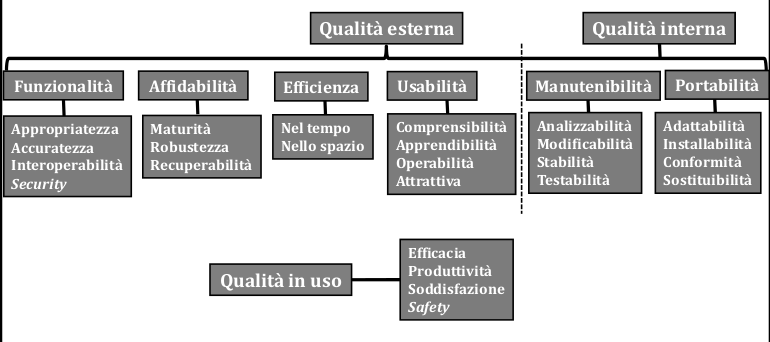
\includegraphics[width=0.78\textwidth]{img/9126}
				\caption{Le diverse visioni delle qualità di ISO 9126:2001.}
			\end{figure}


		\subsection{STATEMENT COVERAGE}	\label{statementcoverage}	\index{Statement Coverage}
		Strumento che si ricorda quali \textit{statement} il test ha attraversato. Si ha quindi copertura al 100\% quando i test effettuati sull'unità sono sufficienti a eseguire almeno una volta tutti i comandi dell'unità con esito corretto. \\
		(Un esempio di differenza con \underline{\hyperref[branchcoverage]{branch coverage}} su \href{https://stackoverflow.com/questions/14519416/a-difference-between-statement-and-decision-coverage}{StackOverflow}).


		\subsection{STATO} \index{Stato} \label{stato}
		%[Da Automi] \\
		È il valore assunto da variabili di stato, conseguente ad azioni precedenti su di esse. Viene deciso dal \textit{Software Engineer}.

		\subsection{STUB}	\index{Stub}	\label{stub}
		Sono dei sostituti (come i \underline{\hyperref[mock]{mock}}), ovvero rappresentano ciò che è chiamato dal test, ma che ancora non c'è (per esempio evita ClassNotFound).

		\subsection{STUDIO DI FATTIBILITÀ} \index{Studio di fattibilità} \label{studiofattibilita}
		Non è un documento pubblico, ma deve rimanere agli atti come un ragionamento ben fondato.
		È quindi un prodotto interno e definisce il rapporto tra le parti. \\
		Si capisce qui cosa si è capaci di fare, perché innanzitutto si valutano rischi, costi e benefici nell'ottica del cliente e del fornitore.
		Si valuta se procedere, con l’obiettivo di restare entro un costo massimo prefissato e con le conoscenze immediatamente disponibili o un piano di formazione.
		Si studiano:
		\begin{itemize}
			\item Gli strumenti e le tecnologie per la realizzazione
			\item Le soluzioni algoritmiche e architetturali
			\item Le piattaforme idonee all'esecuzione
			\item Il costo di produzione rispetto alla redditività
		\end{itemize}
		Inoltre le attività che vengono fatte sono:
		\begin{itemize}
			\item Individuazione dei rischi
			\item Valutazione delle scadenze temporali (con conseguente studio delle risorse disponibili rispetto a quelle necessarie)
			\item Valutazione delle possibili strategie alternative
		\end{itemize}
